\documentclass[a4paper, 11pt, oneside]{report}

\usepackage[T1]{fontenc}    % fornisce la codifica adatta per il font della lingua italiana
\usepackage[utf8]{inputenc} % interpreta i caratteri immessi dall'editor, come i caratteri accentati italiani
\usepackage[italian]{babel} % convenzione per date, capitolo invece di chapter, regole di formattazione...

\usepackage{geometry}       % gestisce il layout del documento
% heightrounded modifica le regole di contenimento del testo per far rientrare il testo in un numero finito di righe
\geometry{a4paper, top=2cm, bottom=2cm, left=2.5cm, right=2.5cm, heightrounded}

\pagestyle{plain}           % numeri di pagina in fondo

\usepackage{hyperref}       % usato per collegamenti ipertestuali
\usepackage{graphicx}       % usato per inserire immagini
\hypersetup{hidelinks}      % usato per rimuovere i riquadri dai link

% autostyle adatta lo stile delle citazioni alla lingua del documento,
% italian=gillments racchiude tra le virgolette caporali i campi che prevedono le virgolette
\usepackage[autostyle,italian=guillemets]{csquotes}
% usato per la generazione rif bibliografici, richiede l'uso di babel e csquotes, biblatex è il motore usato.
% Le citazioni sono definite in termini di etichette numeriche come [1],[2],...
\usepackage[bibstyle=numeric, citestyle=numeric-comp]{biblatex}

\usepackage{quoting}        % usato per citazioni
\usepackage{algpseudocode}  % usato per scrivere pseudo codice
\usepackage{algorithm}
\usepackage{amsmath}
\usepackage{amssymb}

\usepackage{sidecap}        %aggiungere didascalie alle immagini

% preambolo
\title{
\includegraphics[width=0.4\textwidth]{logo}\\WeatherStyle\\Corso Fondamenti di Intellingenza Artificiale\\Prof. F.Palomba}
\author{Repository github:\\\url{https://github.com/frankzamma/NC22_WeatherStyle_classe03.git}\\\\
        \\Aurucci Raffaele\\Miglino Annalaura\\Palmieri Angelo\\Zammarrelli Francesco Giuseppe}
\date{}

\begin{document}

    % sezione dedicata al preambolo
    \begin{titlepage}
        \maketitle
    \end{titlepage}

    % produzione dell'indice automatica
    \tableofcontents

    \part{Introduzione}
        \chapter{Cos'è WeatherStyle?}
            WeatherStyle è un progetto che racchiude un sogno che è quello di cercare di mitigare una delle conseguenze
            dei cambiamenti climatici che affligge le persone ogni giorno: vestirsi in maniera adeguata alle condizioni
            meteorologiche previste.

            \section{Le motivazioni}
            Il progetto Weather Style nasce dall'idea di 4 studenti pendolari dell'Università degli Studi di Salerno per
            risolvere uno dei principali problemi che si trovano ogni giorno ad affrontare.\\
            In particolare, essi si spostano dalla loro residenza per andare
            a seguire corsi (o svolgere esami) presso il Campus di Fisciano e devono scegliere l'abbigliamento
            che sia più adatto per fronteggiare le condizioni climatiche previste.
            Il problema esposto non riguarda solo gli studenti ma anche tutti coloro che devono spostarsi per lavoro
            verso un'altra città, quindi un applicativo che lo risolva, seppur parzialmente,
            potrebbe aiutare un significativo numero di persone.

            \section{Gli obbiettivi}
            L'obiettivo che Weather Style vuole raggiungere è quello di creare un agente intelligente che riesca a fornire
            all'utente dei suggerimenti sui capi d'abbigliamento che ritiene più adatti, questo basandosi su alcune informazioni
            metereologiche come la temperatura percepita, il clima e la stagione in cui è effettuata la previsione.

            \bigskip
            \section{Specifiche PEAS}
            L'acronimo PEAS sta per: Performance Environment Actuators Sensors, e viene utilizzato per descrivere un ambiente.
            \begin{itemize}
                \item \textbf{P (Performance)}: è la misura di prestazione adottata per valutare l'operato di un agente.
                Nel caso di WeatherStyle, la misura di prestazione è data dal consigliare in maniera adeguata i vari capi
                d'abbigliamento.
                \item \textbf{E (Environment)}: è la descrizione degli elementi che formano l'ambiente. Nel nostro
                sistema, l'ambiente è costituito da un insieme di capi d'abbigliamento e dalle previsioni meteo.
                \item \textbf{A (Actuators)}: servono all'agente per poter compiere delle azioni. L'agente di WeatherStyle
                si serve di uno schermo per mostrare all'utente i capi d'abbigliamento che ritiene più adeguati.
                \item \textbf{S (Sensors)}: sono i sensori attraverso i quali l'agente riceve gli input dall'esterno. In
                questo caso, un sensore è sicuramente la tastiera per poter inserire dei capi d'abbigliamento, e le
                informazioni metereologiche.
            \end{itemize}


            \subsection{Caratteristiche dell'ambiente}
                \begin{itemize}
                    \item \textbf{Tipo di ambiente:} guardaroba con informazioni meteorologiche.
                    \item \textbf{Completamente osservabile:} l'agente attraverso i sensori conosce lo stato
                    completo dell'ambiente in ogni momento, ovvero, ha visione completa dei capi presenti nel guardaroba
                    e delle informazioni meteorologiche.
                    \item \textbf{Deterministico:} lo stato successivo dell'ambiente è completamente determinato dallo
                    stato corrente e dall'azione eseguita dall'agente, dunque, è un ambiente che non cambia nel tempo.
                    \item \textbf{Episodico:} l'esperienza dell'agente si divide in episodi atomici, in ogni episodio
                    esegue una singola azione e non si lascia influenzare da ciò che è accaduto precedentemente.
                    \item \textbf{Statico:} l'ambiente non cambia nel mentre che l'agente sta eseguendo le proprie azioni.
                    \item \textbf{Discreto:} l'ambiente fornisce un numero limitato di percezioni\footnote{input percepiti
                    in un dato istante} e azioni distinte\footnote{una sola azione per ogni episodio}.
                    \item \textbf{Singolo agente:} l'ambiente consente la presenza di un singolo agente\footnote{nei
                    capitoli successivi vedremo tre agenti che agiranno singolarmente con uno scopo comune}
                \end{itemize}

    \part{Tecniche di risoluzione}
        \chapter{La ricerca locale}
        Gli algoritmi di \textbf{ricerca locale} a differenza degli algoritmi di ricerca tradizionale non hanno come scopo
        quello di trovare una sequenza di azioni che porti dallo stato iniziale allo stato obbiettivo, bensì lo stato
        obbiettivo rappresenta esso stesso la soluzione al problema, indipendentemente da come ci si è arrivati.
        \par \noindent Questo rende gli algoritmi di ricerca locale particolarmente adatti a problemi di configurazione
        e/o di ottimizzazione. Sono anche detti algoritmi di ``miglioramento iterativo'', poiché partono da un'ipotetica
        soluzione con lo scopo di migliorarla, secondo quella che viene chiamata \textbf{funzione obbiettivo}, una misura
        che serve all'algoritmo per comprendere se e quanto sta migliorando nelle iterazioni, condizione fondamentale per
        la corretta terminazione dell'algoritmo.
        \par \noindent In ultimo accenniamo al fatto che le soluzioni ottenute non sempre sono soluzioni ottimali, ma il
        più delle volte soluzioni sub-ottimali, ciò è dovuto dalla mancata esplorazione dell'intero spazio degli stati;
        compito del progettista è cercare di migliorare la capacità di esplorazione dell'algoritmo.

            \section{Gli algoritmi genetici}
            Sebbene possa sembrare un argomento che si sia affacciato da poco sull'umanità, la storia degli algoritmi genetici
            ha inizio con il celeberrimo biologo inglese, Charles Darwin.
            \par \noindent Darwin pubblicò nel 1859 \textit{"L'origine della specie"}, libro che riscosse un enorme
            successo e nel quale si introduceva per la prima volta il concetto di \textbf{teoria dell'evoluzione} tramite
            un processo di \textbf{selezione naturale}.
            \par \noindent Negli anni '50 del XX secolo cominciò il diffondersi degli algoritmi evolutivi,
            i quali usano tutti i concetti formulati dalla teoria di Darwin, ovvero:
            \textit{genotipo}, \textit{fenotipo}, \textit{individuo}, \textit{popolazione}, \textit{evoluzione} e via dicendo.
            \par \noindent
            \\ \noindent Tra l'insieme degli algoritmi evolutivi troviamo anche gli \textbf{algoritmi genetici} che vennero
            presentati nel 1975 da John Holland, all'epoca detti \textit{genetic plans}.
            \par \noindent La definizione di algoritmi genetici è dunque la seguente:
            procedura di alto livello (meta-euristica) ispirata alla genetica per \textbf{definire}
            un algoritmo di ricerca.
            \par \noindent
            \\ \noindent Partendo da questa definizione si può dire che un algoritmo genetico evolve una \textbf{popolazione}
            di \textbf{individui} (le cosiddette soluzioni candidate) producendo un iterazione dopo l'altra delle
            soluzioni che migliorino sempre rispetto ad una \textbf{funzione obbiettivo}, fino a che non si è raggiunta
            la soluzione \textbf{ottimale} o si sia verificata una \textbf{condizione di terminazione}.
            Per poter creare nuove \textbf{generazioni} di individui bisogna applicare degli \textbf{operatori genetici},
            più nello specifico la \textbf{selezione}, il \textbf{crossover} e la \textbf{mutazione}.
            \par \noindent

            \newpage
            \section{Formulazione del problema}
            Il primo quesito da porsi nel momento in cui si ha a che fare con un algoritmo genetico è: come vengono
            codificati gli individui? Nel nostro caso, l'algoritmo dovrà scegliere solamente tre dai capi che si ritengono
            più adeguati; per questo motivo, la codifica degli individui consiste in un array di tre interi. Questi ultimi
            rappresentano la posizione del capo d'abbigliamento scelto nella lista di tutti i capi.
            \par \noindent Dopo aver definito come gli individui devono essere codificati, si passa ad analizzare i vincoli a
            cui essi sono sottoposti. In questo caso, l'unico vincolo è che, all'interno dell'array, non si ripeta un intero
            più di una volta, cioè che i capi siano tutti diversi tra loro.
            \par \noindent La prima parte di un GA consiste nell'inizializzazione di una popolazione. Inizialmente la soluzione
            verteva verso un'inizializzazione casuale ma, dopo aver constatato che la popolazione non rispettava il vincolo richiesto,
            si è pensato a un'inizializzazione pseudo-casuale, cioè producendo array ammissibili (che rispettino il vincolo citato sopra)
            contrastando il fatto che un elemento si possa ripetere più volte.
            \\ \noindent Dopo aver chiarito la codifica degli individui, bisogna modellare la funzione di fitness.
            Il nostro obiettivo è quello di fornire all'utente la selezione dei tre capi migliori in base alle condizioni meteo; per
            ogni capo d'abbigliamento, viene calcolato un punteggio (utilità) che consente di aiutare l'agente nella scelta.
            \par \noindent Il punteggio si basa su diversi parametri:
            \begin{itemize}
                \item \textbf{Temperatura.} Sono stati differenziati ben sette range di temperatura in cui, per ognuno,
                vengono assegnati i punteggi ai vari materiali di cui può essere composto un capo d'abbigliamento (maglie e pantaloni).
                Ad esempio, quando la temperatura scende al di sotto dei cinque gradi, verrà assegnato un punteggio maggiore ad un tessuto
                come la lana piuttosto che ad uno come il lino, essendo tipicamente estivo. Per le scarpe viene, inoltre, incrementato il
                punteggio anche sulla base della pioggia: se le previsioni metereologiche dichiarano pioggia, verranno assegnati punti "bonus"
                se la scarpa è antiscivolo e/o impermeabile.
                \item \textbf{Lunghezza.}Nei range suddetti vengono anche specificati i punteggi relativi
                alla lunghezza sia dei pantaloni che delle maglie relativamente alla manica; tenendo in considerazione l'esempio precedente, verrà
                sicuramente preferita una manica lunga e un pantalone lungo rispetto alle altre lunghezze.
                \item \textbf{Stagionalità.} Inoltre, si assegna una valutazione sulla base della stagionalità del capo; sia per le maglie, che per i
                pantaloni e per le scarpe, viene dato il massimo del punteggio se la stagione in cui viene richiesto l'intervento dell'agente coincide
                con quella indicata per quel determinato capo d'abbigliamento.
                \item \textbf{Tipo di scarpe.} In base alle previsioni meteo e al tipo di scarpe, viene assegnato un determinato punteggio. Ad esempio,
                in caso di neve, vengono preferiti gli stivali alle classiche scarpe di ginnastica.
                \item \textbf{Colore.} Si tende, per ognuna delle tre tipologie di capo d'abbigliamento, a preferire colori chiari in caso di meteo
                soleggiato piuttosto che colori scuri; per i capi colorati, i punti corrispondono a cinque, esattamente a metà tra i dieci per i capi
                chiari e zero per quelli scuri.
            \end{itemize}
            \\ \noindent Riassumendo, per ogni capo d'abbigliamento si calcola la sua utilità. In particolare, per maglie e pantaloni, l'utilità
            è data da \textit{u(x)=te(x)+c(x)+l(x)+s(x)}, dove \textit{te(x)} rappresenta la temperatura, \textit{c(x)} il colore, \textit{l(x)}
            la lunghezza, \textit{s(x)} la stagionalità. Allo stesso modo, per le scarpe l'utilità è espressa come \textit{u(x)=ti(x)+te(x)+s(x)+c(x)},
            in cui \textit{te(x)}, \textit{c(x)} e \textit{s(x)} assumono lo stesso significato detto in precedenza, e \textit{ti(x)} rappresenta il tipo
            di scarpa.
            \ \noindent In conclusione, la funzione di fitness è data dalla media dei tre punteggi assegnati ad ogni capo d'abbigliamento, cioè
        \begin{equation*}
            \frac{\sum_{n=1}^{3} u_{n}}{3}
        \end{equation*}


            \newpage
            \section{Implementazione}
            Per l'implementazione della soluzione basata su algoritmo genetico è stato utilizzato il framework
            \textbf{Jenetics} \cite{1}.
                \subsection{Codifica degli individui}
                \par \noindent Per prima cosa è stato necessario definire come è fatto un individuo, secondo la logica
                del framework quando si parla di individuo, esso è chiamato \textbf{Genotype}, a sua volta composto
                da cromosomi, detti \textbf{Chromosome}, i cromosomi a loro volta sono costituiti da geni, detti
                \textbf{Gene}.
                \medskip
                \par \noindent Rispetto a ciò che è stato detto nella sezione \ref{codifica:ga} possiamo definire
                i genotipi mediante tre cromosomi, costituti da geni che a loro volta hanno al proprio interno valori
                interi che variano da \textbf{0} a \textbf{sizeCapi $-$ 1}.
                \medskip
                \begin{algorithmic}[1]
                    \State $firstChromosome \gets Gene(0,sizeCapi-1)$
                    \State $secondChromosome \gets Gene(0,sizeCapi-1)$
                    \State $thirdChromosome \gets Gene(0,sizeCapi-1)$
                    \State $genotype \gets [firstChromosome, secondChromosome, thirdChromosome]$
                \end{algorithmic}

                \subsection{Vincoli}
                \par \noindent Per quel che riguarda la definizione dei vincoli già discussi nella sezione \ref{vincoli:ga}
                il framework mette a disposizione l'interfaccia \textbf{Constraint} attraverso la quale si vanno a ridefinire
                due metodi:
                \begin{itemize}
                    \item \textbf{test():} metodo che verifica se un genotipo ottenuto in una qualsiasi iterazione è un
                    buon individuo o meno.
                    Nello specifico diremo che il test ha avuto esisto positivo se i valori interi di cui è composto il
                    genotipo sono tre valori diversi, altrimenti diremo che ha avuto esito negativo.
                    \item \textbf{repair():} metodo che viene chiamato quando un genotipo non ha superato il test e si
                    cerca quindi di ripararlo.
                    Nello specifico andremo a costruire un nuovo genotipo che rispetta il vincolo e lo assoceremo a un
                    \textbf{Phenotype}, ovvero un individuo che è stato valutato; esso viene passato in input al metodo
                    ed è costituito dal valore di fitness ottenuto e da un numero \emph{i}, ovvero la i-esima generazione
                    a cui appartiene.
                \end{itemize}

                \subsection{Funzione di fitness}
                \par \noindent Venendo alla funzione di fitness, come già descritto nella sezione \ref{fitness:ga} il
                nostro obbiettivo è quello di massimizzare il punteggio ottenuto dalla combinazione dei geni per ogni
                fenotipo.
                \par \noindent In termini semplici, per ogni individuo andremo a valutare i tre valori interi, i quali
                corrisponderanno alle posizioni dei capi d'abbigliamento in una lista, calcoleremo il punteggio per ognuno,
                faremo una media e restituiremo il risultato.

                \subsection{Operatori genetici}
                Per la risoluzione del problema sono stati scelti i seguenti operatori genetici:
                \begin{itemize}
                    \item \textbf{RouletteWheelSelector:} operatore di selezione, gli individui ricevono una probabilità
                    di selezione calcolata includendo il corrispettivo valore di fitness. L'algoritmo andrà a selezionare
                    $n$ individui, saranno consentite ripetizioni degli stessi individui.
                    \item \textbf{MultiPointCrossover:} operatore di crossover, selezionerà due punti casuali in ogni
                    individuo, scambierà il patrimonio genetico di quest'ultimi a coppie di due rispetto ai punti di
                    crossover e genererà per ogni coppia di genitori due nuovi individui figli che costituiranno la
                    successiva generazione. È stata inoltre inserita una probabilità di crossover pari a $0.25$.
                    \item \textbf{GaussianMutator:} operatore di mutazione, muterà casualmente un gene dall'individuo
                    risultante dell'applicazione del crossover, il valore del nuovo gene sarà calcolato prendendo un
                    valore definito nella distribuzione gaussiana a partire dal gene corrente.
                \end{itemize}

                \subsection{Setup dell'algoritmo}
                Dopo aver quindi dato una codifica agli individui, definiti i vincoli, la funzione di fitness e aver
                scelto gli operatori genetici è giunta l'ora di fare il setup dell'algoritmo.
                \par \noindent Nel seguente pseudo codice riassumiamo i passi fondamentali.
                \medskip
                \begin{algorithm}
                \caption{Setup genetic algorithm}
                    \label{setup:ga}
                    \begin{algorithmic}[1]
                        \State $populationSize \gets 10$
                        \State $maxEvaluation \gets 100$
                        \State
                        \State $constraint \gets ConstraintImplement()$
                        \State $selector \gets RouletteWheelSelector()$
                        \State $crossover \gets MultiPointCrossover(0.25)$
                        \State $mutator \gets GaussianMutator()$
                        \State
                        \State $geneticAlgorithm \gets setup(populationSize, maxEvaluation, genotype, fitness,$
                        \State $\hspace*{12.3em} constraint, selector, crossover, mutator)$
                    \end{algorithmic}
                \end{algorithm}

            \section{Vantaggi e svantaggi}
            La soluzione illustrata in questo capitolo presenta dei vantaggi e degli svantaggi, molti dei quali legati
            alla natura degli algoritmi genetici.
            Uno dei principali problemi affrontati è stato sulla generazione della popolazione iniziale.
            In genere, la prima popolazione viene generata in maniera totalmente casuale quindi non è detto che
            tali individui rispettino il vincolo imposto (i tre elementi devono essere diversi).\\
            Il problema è stato risolto andando ad impostare una generazione pseudo casuale che permette
            di avere anche nella prima generazione degli elementi ammissibili e, di conseguenza,
            la ricerca viene guidata verso soluzioni ammissibili e migliori riducendo il carico computazionale.\\
            A valle di test empirici, possiamo dire che la soluzione riesce quasi sempre a restituire un risultato ottimale.
            In particolare, su 10 test effettuati ben x volte il risultato è da considerare ottimo.
            Di seguito un report del test eseguito:\\
                \begin{tabular}{ |p{3cm}|p{2cm}|p{2cm}||p{4cm}|}
                    \hline
                    \multicolumn{4}{|c|}{Test effettuati} \\
                    \hline
                    Data previsione & Meteo & Temperatura Percepita & Risultato\\
                    \hline
                    11/09/2022 & piovoso  & 11 & x\\
                    \hline
                    02/12/2022 & nuvoloso  & 13 & x\\
                    \hline
                    04/04/2022 & piovoso  & 18 & x\\
                    \hline
                    01/02/2022 & soleggiato  & 3 & x\\
                    \hline
                    13/01/2022 & neve  & 5 & x\\
                    \hline
                    20/02/2022 & soleggiato  & 20 & x\\
                    \hline
                    16/04/2022 & piovoso  & 15 & x\\
                    \hline
                    6/08/2022 & Nuvoloso  & 30 & x\\
                    \hline
                \end{tabular}
            \subsection{Efficienza}\label{subsec:efficienza}
            Un'osservazione importante da fare riguarda l'efficienza.
            Con un guardaroba di grandi dimensioni, gli algoritmi genetici,
            ci permettono sicuramente di effettuare un numero inferiore di computazioni rispetto ad una ricerca esaustiva
            restituendo quasi sempre buon risultato.
            Tuttavia, con il setup da noi effettuato, cioè \emph{size della popolazione = 10} e
            \emph{max= 100}, i GA diventano più efficienti di una ricerca esaustiva con un numero di capi
            maggiore o uguale a 20.
            Infatti, facendo un po' di calcoli il numero stati ammissibili con 20 capi è pari al numero di combinazioni semplici
            di 20 elementi raggruppati in classi di 3:
            \begin{equation*}
                C_{20,3}=\binom{20}{3}= 1120
            \end{equation*}
            che è leggermente superiore al numero massimo di valutazione della funzione di fitness che il GA compie durante la sua esecuzione:
            \begin{equation*}
                populationSize * maxEvaluation = 10 * 100 = 1000
            \end{equation*}
            Bisogna però sottolineare, che la precedente osservazione considera che la ricerca esaustiva venga effettuata soltanto
            tra i possibili stati ammissibili per la soluzione, che richiedono anche essi una computazione per essere generati.
            Quindi, ritrattando, se consideriamo tutte le soluzioni (ammissibili e non ammissibili) i GA diventano più efficienti già a partire da
            11 capi d'abbigliamento:
            \begin{equation*}
                D_{11,3}^{'}=11^3 = 1331  > 1000 = populationSize * maxEvaluation = 10 * 100 = 100
            \end{equation*}
            Per concludere, la soluzione basata su Algoritmi Genetici, riesce a fornire un buon consiglio all'utente
            in quasi tutte le condizioni meteo.
            In alcuni casi, essi hanno restituito un risulto sub-ottimo in cui, ad esempio, uno dei tre dei capi non era
            particolarmente adatto, ma essendo che la scelta tra i tre è effettuata dall'utente, si ritiene che tale soluzione
            sia applicabile nel sistema finale, eventualmente effettuando un raffinamento della funzione di fitness per
            evitare i casi di risultati sub-ottimi.


    \chapter{Il machine learning}
        Quando si parla di \textbf{machine learning} solitamente si tende ad accomunarlo al concetto di ``Intelligenza Artificiale'',
        ma (s)fortunatamente non è così.
        \par \noindent Il machine learning altro non è che una branca dell'Intelligenza Artificiale, una delle forme
        di apprendimento automatico con origini più antiche, sin nei tardi anni 50 Alan Turing avanzò la proposta
        di realizzare algoritmi per costruire macchine in grado di apprendere.
        \par \noindent \textbf{Dunque in cosa consiste?} Sostanzialmente è lo studio degli algoritmi e delle tecniche in
        grado di apprendere dai dati.
        Si discosta moltissimo da quella che è la classica programmazione\ldots quando si effettua machine learning non
        è più il programmatore a scrivere la funzione $f(x)$ con input e output ben definiti, ma il
        programmatore dovrà semplicemente preoccuparsi di fornire i dati ad un algoritmo di addestramento che sulla base
        di questi costruirà un modello in grado di fare delle predizioni. A loro volta queste predizioni sono fornite
        mediante un ulteriore algoritmo dopo aver dato in pasto degli input al modello addestrato.
        \\
        \par \noindent Ci sono diversi modi di fare machine learning, in questo capitolo ci concentreremo sull'
        \textbf{apprendimento supervisionato}, ovvero problemi in cui bisogna fornire ad un algoritmo di addestramento
        dati etichettati, ovvero osservazioni in cui sia disponibile la variabile dipendente: il valore che
        dovrà essere in grado di predire il modello una volta addestrato.
        In particolare i nostri sforzi saranno incentrati sugli algoritmi di \textbf{regressione}, ovvero tecniche in grado
        di predire il valore di una variabile numerica sulla base degli input forniti.

            \bigskip
            \section{CRISP-DM}
            Per progettare una soluzione basata sul \textbf{machine learning} bisogna avere un approccio data \& software
            engineering.
            Questo è necessario perché la stragrande maggioranza dei sistemi software che non sono adeguatamente ingegnerizzati
            falliscono e rischiano di arrecare danni a cose, persone e ambiente circostante.
            \par \noindent Per avere un corretto approccio ingegneristico è possibile scegliere uno dei vari cicli di vita
            di progetti basati su intelligenza artificiale e data science, uno dei più conosciuti è il CRISP-DM ed è anche
            il modello che abbiamo adottato noi per progettare la nostra soluzione.
            \par \noindent
            \\ \noindent Il CRISP-DM (Cross-Industry Standard Process for Data Mining) è formato da diverse fasi che possono
            essere eseguite un numero illimitato di volte il che lo rende un modello \textit{non} sequenziale.
            Nelle sezioni che seguono andremo ad analizzare le fasi del CRISP-DM, mostrando cosa è stato fatto in ognuna di esse
            al fine di poter raggiungere il nostro obiettivo tramite una soluzione basata sul machine learning.
            \par \noindent
            \begin{center}
                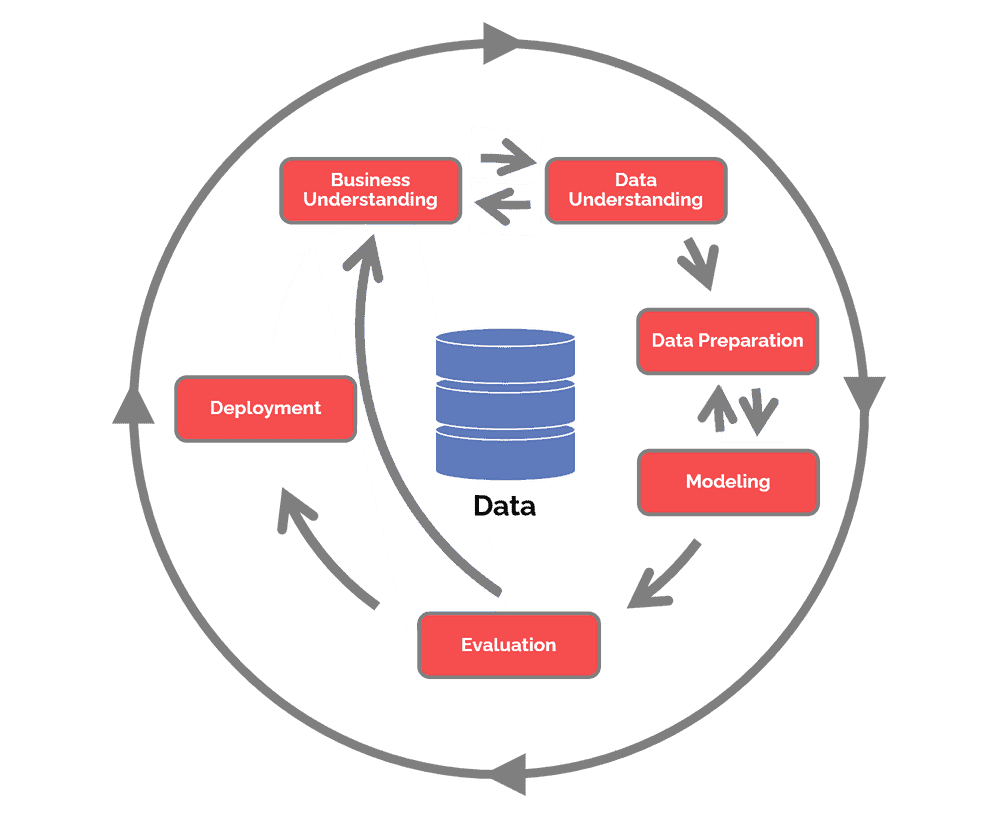
\includegraphics[scale=0.3]{CRISP-DM}
            \end{center}

            \section{Business Understanding}
            La prima fase del CRISP-DM è quella di \textbf{Business Understanding}.
            Qui si raccolgono i requisiti e si definiscono gli obiettivi di business che si intende raggiungere, oltre a
            determinare la disponibilità delle risorse, stimare i rischi, indicare le tecnologie e gli strumenti utilizzati
            per raggiungere gli obbiettivi di business.
            \par \noindent
            \begin{itemize}
                \item \textbf{Obiettivi di business}: Il machine learner che stiamo progettando avrà come obiettivo quello di
                saper stimare adeguatamente, attraverso un punteggio numerico, quali capi d'abbigliamento sono più adatti basandosi
                sulle caratteristiche dei capi e sulle informazioni metereologiche quali temperatura percepita, clima e
                stagione della previsione.
                \item \textbf{Disponibilità delle risorse}: Per raggiungere il nostro obbiettivo principale ci serviranno
                delle risorse ovvero un dataset per ogni capo d'abbigliamento (maglia, pantalone e scarpa),
                che contiene informazioni riguardo il capo d'abbigliamento specifico e delle informazioni meteo correlate.
                \par \noindent Purtroppo dopo un'approfondita ricerca non siamo riusciti a trovare nessun dataset che facesse
                al caso nostro, anche sfruttando piattaforme importanti nell'ambito del machine learning come \textbf{Kaggle} \cite{3},
                quindi per rimediare a questo abbiamo costruito i dataset che ci servivano acquisendo, analizzando e modellando
                i dati da altri dataset.
                \item \textbf{Stima dei rischi}: Il non avere già in partenza dei dataset su cui poter lavorare comporta
                di certo un rischio non di poco conto dato che bisogna costruirseli da se e dunque i dati non sono adeguatamente testati.
                \item \textbf{Tecnologie e strumenti}: Per acquisire, analizzare e modellare i dati abbiamo scelto di utilizzare
                il linguaggio Python poiché mette a disposizione alcune librerie come \textbf{pandas} \cite{4} e \textbf{seaborn} \cite{5}.
                L'addestramento e l'implementazione dei modelli invece è stata realizzata in linguaggio Java,
                sfruttando il framework \textbf{Weka} \cite{2}, questo per comodità dato che l'intero applicativo di Weather Style
                è scritto usando tale linguaggio di programmazione.
            \end{itemize}

            \newpage
            \section{Data Understanding}
            Come già discusso durante la fase di business understanding il principale rischio dell'approccio basato su machine
            learning è stato l'effettiva mancanza di un dataset che rispondesse appieno alle nostre esigenze.
            \par \noindent Ciononostante abbiamo trovato diversi dataset che in un qualche modo fusi insieme hanno potuto
            dar vita al dataset di cui avevamo bisogno, e in buona parte ci siamo riusciti!
            \par \noindent In questa sezione andremo quindi ad acquisire i dati, visualizzarli, analizzarli e documentarli rispetto al loro
            formato e alla loro qualità.
                \subsection{Dataset maglie e pantaloni}
                La prima cosa da fare quindi era trovare un dataset che comprendesse i dettagli di diversi capi d'abbigliamento,
                Github si è dimostrato di grande aiuto e il dataset \cite{6} corrispondeva a ciò di cui avevamo bisogno.
                \\
                \par \noindent Il dataset contava più di $14000$ osservazioni.
                \\
                \par \noindent La feature che ci ha permesso di distinguere la tipologia dei capi d'abbigliamento
                era indicata come \textit{Type} i cui valori unici erano \textbf{Top}, \textbf{Bottom} e \textbf{Dress}.
                Per il nostro problema non sono stati considerati i vestiti da donna, quindi nella fase di data preparation
                ne terremo conto.
                \begin{center}
                    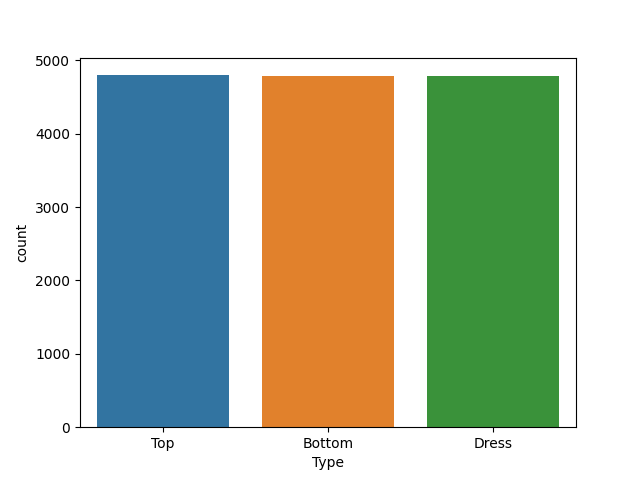
\includegraphics[scale=0.4]{countTopBottom}
                \end{center}
                \bigskip
                \par \noindent Tra le altre feature molto interessanti presenti nel dataset rientra anche la stagione
                in cui il capo d'abbigliamento è indicato, la colonna corrispondente è denominata \textit{Season}.
                Qui notiamo molte categorie distinte per la stagione che potremmo eventualmente generalizzare.
                \begin{center}
                    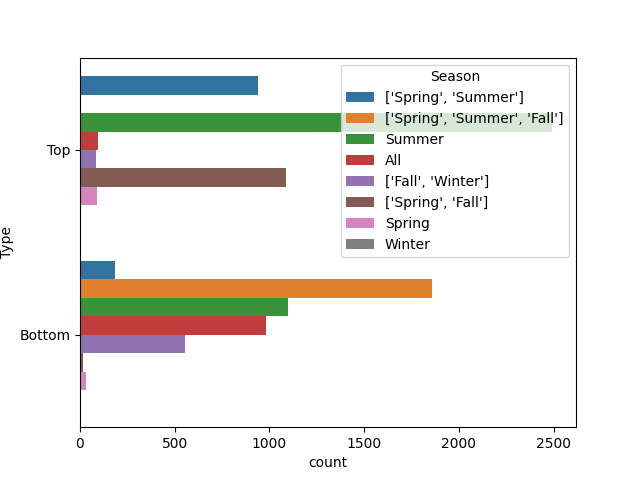
\includegraphics[scale=0.4]{countSeasonTopBottom}
                \end{center}
                \newpage
                \par \noindent Altra feature importante presente nel dataset è quella indicata come \textit{Material}
                dove vanno per la maggiore i capi in \textbf{Cotton} e \textbf{Polyester}. Da non trascurare la presenza
                di tanti materiali di tipologia diversa e di come questi potrebbero essere generalizzati, ad es: \textbf{Cotton Blends}
                è possibile generalizzarlo nella categoria Cotton.
                \begin{center}
                    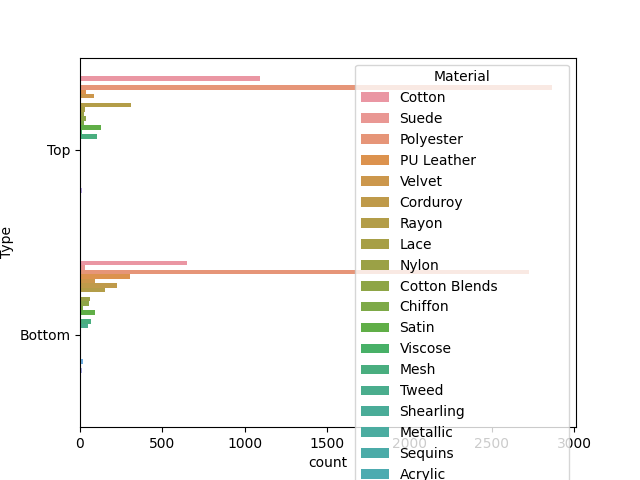
\includegraphics[scale=0.4]{countMaterialTopBottom}
                \end{center}
                \bigskip
                \par \noindent \textit{Color} è un'altra feature di cui abbiamo fatto uso per costruire il dataset. Avendo,
                però, definito il colore in tre macrocategorie (chiaro, scuro e colorato), è diventata necessaria effettuare
                un'operazione di smistamento dei vari colori nelle relative macrocategorie.
                \\ \noindent Infine come ultima feature molto importante presente nel dataset per quanto riguarda i capi
                d'abbigliamento della categoria \textbf{Top} è la colonna indicata come \textit{Sleeve Length}. Si può
                notare come per la maggior parte siano presenti maglie della categoria \textbf{Loong Sleeve} e
                \textbf{Short Sleeve}.
                \begin{center}
                    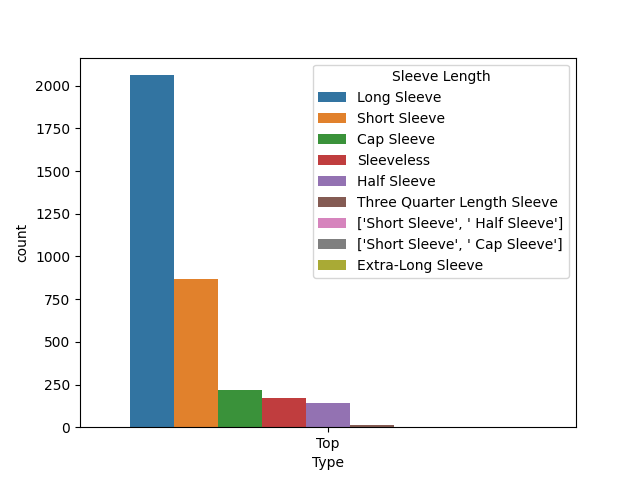
\includegraphics[scale=0.4]{countLengthTop}
                \end{center}
                \subsection{Dataset scarpe}
                Il dataset illustrato al punto precedente, non contiene informazioni in merito alle scarpe.
                Per fortuna, su \cite{3} è disponibile  \cite{7} che ci ha permesso di andare avanti con il nostro lavoro.
                \\
                Il dataset contava $50025$ record di scarpe.
                \\
                Molte di queste righe, hanno, però dei valori nulli.
                Eliminando tali righe si scende a $18260$ record.\\
                Inoltre, il dataset ripulito dai valori nulli presenta molti duplicati, eliminandoli si scende a $7323$ record distinti.\\
                Il dataset presenta i seguenti attributi:
                \begin{itemize}
                    \item CID : colonna che costituisce l'id dei record
                    \item Category: categorie delle scarpe
                    Nel seguente grafico si può vedere che sono presenti 4 categorie:
                    \begin{center}
                        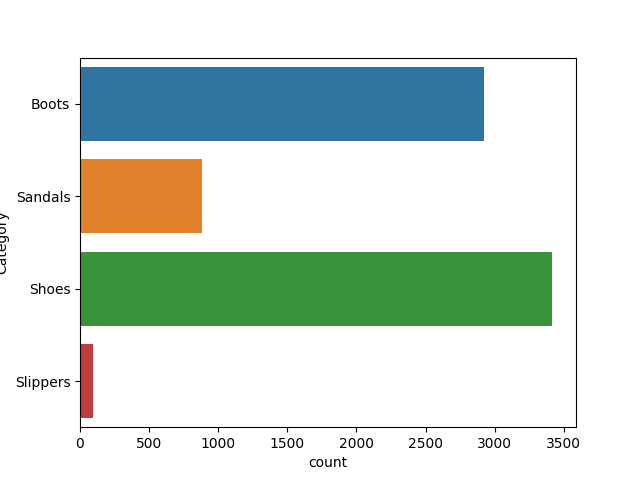
\includegraphics[scale=0.4]{CategoryShoes}
                    \end{center}
                    \item SubCategory: sotto-categorie delle scarpe.
                    Sono presenti diverse categorie di scarpe:
                    \begin{center}
                        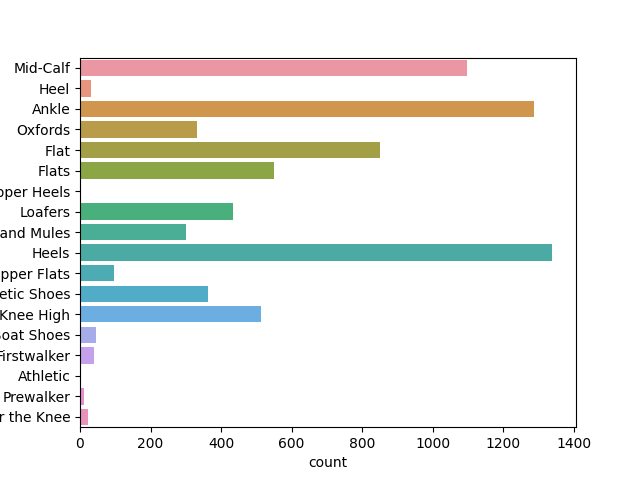
\includegraphics[scale=0.4]{SubCategoryShoes}
                    \end{center}
                    \item HeelHeight: Altezza del tacco in pollici.
                    Questa caratteristica è poco interessante per i nostri obiettivi
                    \item Insole: Materiale della suola.
                    Anche questa caratteristica, è poco utile ai nostri scopi perché per nella realtà tale dato sarà
                    difficilmente disponibile a meno che una persona sia un esperto di scarpe.
                    Tuttavia, nella fase di data preparation ci ritornerà utile per imputare un'altra caratteristica.
                    \item Closure: rappresenta il modo in cui viene chiusa la scarpe (Eg. Lacci, Strappi).
                    Neanche questa caratteristica ci aiuta a raggiungere i nostri obiettibi
                    \item Gender: rappresenta il genere a cui è rivolta la scarpa.
                    Questo oltre a servire poco per i nostri, può essere considerato un attributo sensibile e,
                    di conseguenza, verrà eliminato nella fase successiva,
                    \item Material: Il/i materiale/i di cui è composta la scarpa.
                    Poco utile, considerazioni simili a quelle fatte per la Insole.
                    \item ToeStyle: stile della punta.
                    Anche questo attributo ci aiuta poco.
                \end{itemize}
                \subsection{Dataset meteo}
                Per poter consigliare un outfit sulla base delle previsioni meteo, sono ovviamente necessari
                uno o più dataset che contengano questi dati.\\
                Il sito Open-meteo\cite{9} permette di scaricare dati storici delle previsioni meteorologiche.
                Sono molti i dati meteo sia orari che giornalieri che esso fornisce, tuttavia se li utilizzassimo tutti rischieremo di scendere troppo nel dettaglio
                rischiando di non riuscire ad effettuare un predizione.
                Si è deciso di utilizzare, quindi, i dati giornalieri utilizzando le seguenti caratteristiche:
                \begin{itemize}
                    \item \emph{Time}: data a cui si riferiscono i dati meteo;
                    \item \emph{WeatherCode} : codice che indica una condizione meteo (Eg. Piovoso, Soleggiato);
                    \item \emph{Maximum Temperature}  : temperatura massima;
                    \item \emph{Minimum Temperature} : temperatura minima;
                \end{itemize}
                Successivamente, vedendo che le feature \emph{Minimum Temperature} e \emph{Minimum Temperature} non avevano un
                forte potere predittivo, si è deciso di sostituirli con \emph{Minimum Apparent Temperature}
                e \emph{Minimum Apparent Temperature} che indica la temperatura percepita, ovvero la temperatura influenzata dal vento e dall'umidità
                Inoltre, per ottenere un quantità di dati che comprenda più osservazioni possibili abbiamo scelto di scaricare i dati di
                14 città italiane diverse:
                \begin{itemize}
                    \item Aosta
                    \item Belluno
                    \item Cortina
                    \item Firenze
                    \item Fisciano
                    \item Genova
                    \item Milano
                    \item Napoli
                    \item Palermo
                    \item Parma
                    \item Potenza
                    \item Roma
                    \item Salerno
                    \item Treviso
                \end{itemize}
            Nella successiva fase di data preparation, i diversi dataset divisi per città verranno fusi in uno solo.

            \newpage
            \section{Data Preparation}
            In questa sezione tratteremo le tecniche adottate per preparare i dati acquisiti nella fase precedente in
            modo che siano di un formato comprensibile al nostro machine learner.
                \subsection{Dataset maglie e pantaloni}
                Per costruire i dataset contenenti le informazioni delle \textbf{maglie} e dei \textbf{pantaloni} ci siamo serviti delle
                informazioni ricavate nella fase di Data Understanding \textit{(sottosezione 3.3.1)}.
                \par \noindent Il procedimento di \textit{Data Preparation} si articola nei seguenti quattro passaggi:
                \begin{itemize}
                    \item \textbf{Data cleaning}: la cosidetta \textit{"pulizia dei dati"} si occupa di
                    rimediare a problemi che sorgono quando ci sono righe del dataset che hanno dei dati \textbf{mancanti}, ma più
                    in generale ha come obbiettivo quello di fornire un dataset dotato di una \textbf{qualità} ritenuta adeguata
                    per poter procedere con i successivi passaggi.
                    \par \noindent Nel nostro specifico caso abbiamo individuato alcuni dati mancanti in corrispondenza della
                    colonna della \textit{lunghezza della manica} (dataset maglie) e della \textit{lunghezza del pantalone}.
                    \par \noindent Si è scelto, in entrambi i casi sia per il dataset delle maglie che per il dataset
                    dei pantaloni, di non andare a rimuovere le colonne dai due dataset poiché le consideriamo due caratteristiche
                    molto utili per il nostro machine learner nel momento in cui dovrà effettuare delle previsioni.
                    Si è scelto, sempre in ambedue i dataset, di non andare a rimuovere le righe che avevano celle mancanti
                    perché ci si è resi conto che il numero di istanze diminuiva notevolmente.
                    \par \noindent Abbiamo dunque scelto di affidarci al \textbf{data imputation}, insieme di tecniche che
                    possono stimare il valore dei dati mancanti sulla base dei dati a nostra disposizione.
                    Nello specifico abbiamo adottato la tecnica di imputazione \textit{"most frequent imputation"} che permette
                    di sostituire i dati mancanti col valore più frequente contenuto in una colonna.
                    \par \noindent Fatto ciò non si avranno più dati mancanti, successivamente abbiamo riscontrato una grande
                    diversificazione di valori nella colonna relativa al materiale, sia nelle maglie che nei pantaloni.
                    Si è dunque deciso di ricondurre questi valori ad un elenco di materiali più ristretto in modo tale da ridurre
                    la complessità in fase di addestramento e previsione.
                    Ciò è stato possibile poiché abbiamo scelto con cura il nostro elenco di materiali in modo tale che fossero;
                    quelli più comuni sul mercato, facilmente riconoscibili dagli utenti che utilizzeranno l'applicativo e
                    facilmente riconducibili all'elenco di materiali di partenza.
                    \par \noindent Inoltre si è trasformato la colonna dei colori in modo che indicasse se la maglia o il pantalone
                    fosse chiaro, scuro o colorato.
                    Questo perché il nostro obbiettivo \textbf{non} è quello di fornire un punteggio ad un determinato capo andando ad
                    analizzare le varie combinazioni di colori che si possono ottenere.
                    \par \noindent Infine si è tradotto, per una scelta convenzionale, dall'inglese all'italiano ogni valore.
                    \item \textbf{Feature scaling}: Il \textit{feature scaling} è un insieme di tecniche che permettono di
                    normalizzare o scalare l'insieme di valori di una caratteristica.
                    \par \noindent Nel caso della preparazione dei nostri dataset di maglie e pantaloni non è stata effettuata
                    il  \textit{feature scaling} poiché tutte le feature sono di tipo categorico e non numerico.
                    \item \textbf{Feature selection}: Il \textit{feature selection} rientra nell'ambito del \textit{feature engineering},
                    cioè il processo nel quale un progettista usa la propria conoscenza del dominio per determinare le caratteristiche
                    (feature) dai dati grezzi estraibili tramite tecniche di data mining. Il \textit{feature selection} è un processo tramite
                    il quale vengono selezionate le feature più rilevanti per un problema, a partire da un insieme di caratteristiche esistenti.
                    Le feature considerate più rilevanti (sia per le maglie che per i pantaloni) sono:
                    \begin{itemize}
                        \item \textbf{Materiale.} La feature è discriminante, in quanto ci consente di capire se un determinato materiale è adatto per
                        una certa temperatura o meno. Ad esempio, il lino è un tessuto tipicamente estivo, di conseguenza non è indossabile nella
                        stagione invernale.
                        \item \textbf{Colore.} Anche in questo caso, la caratteristica è determinante perché, a parità di meteo soleggiato, bisogna preferire
                        un capo di colore chiaro rispetto a uno di colore scuro.
                        \item \textbf{Lunghezza.} La lunghezza dei pantaloni oppure la lunghezza della manica per le maglie sono rilevanti ai fini della
                        risoluzione del problema; infatti, una manica corta sicuramente sarà da preferire ad una manica lunga se si è in estate.
                        \item \textbf{Stagione.} La feature è rilevante, in quanto viene considerata la differenza tra la stagione in cui viene richiesto il
                        suggerimento e stagionalità del capo: se, ad esempio, il suggerimento viene richiesto a febbraio, sicuramente non verrà considerato
                        un capo dichiarato come "estivo".
                    \end{itemize}
                    \item \textbf{Data balancing}: con \textit{data balancing} si intende l'insieme delle tecniche per convertire un dataset sbilanciato in un
                    dataset bilanciato. Nel nostro caso, abbiamo fatto uso delle tecniche di oversampling per aggiungere righe al dataset.
                    Nel caso delle maglie, essendo che nel dataset di partenza i capi erano prevalentemente estivi, sono state aggiunte più righe per quanto riguarda
                    la stagione invernale, compensando la mancanza di dati nell'insieme di dati iniziale. In maniera del tutto analoga, per i pantaloni sono state
                    generate righe casuali, focalizzando particolarmente l'attenzione su capi invernali. La generazione dei dati, sia per le maglie che per i pantaloni,
                    è stata effettuata con l'ausilio di Google Sheet, tramite la funzione \textit{SCEGLI(CASUALE.TRA...)}, con cui era possibile scegliere un valore a caso
                    tra i valori contenuti nelle celle di riferimento.
                \end{itemize}
                \subsection{Dataset scarpe}
                Il dataset illustrato nella fase di Data Understanding, ci è stato utile per costruire un dataset utilizzabile per il training.
                In particolare, partendo dal ragionamento fatto per la soluzione basata su ricerca, per poter determinare il valore di utilità
                di una scarpa sono necessarie le seguenti caratteristiche:
                \begin{itemize}
                    \item \emph{Tipo}
                    \item \emph{Antiscivolo}
                    \item \emph{Impermeabile}
                    \item \emph{Colore}
                    \item \emph{Stagione}
                \end{itemize}
                Tali caratteristiche non erano immediatamente disponibili, tuttavia si è riusciti a ricavarle durante
                i vari step del  \emph{Data Preparation}:
                \begin{itemize}
                    \item Data Cleaning:\\
                    Come già accennato nel Data Understanding, il dataset contiene molti righe con valori nulli.
                    Ci sono diverse tecniche di Data Imputation che permettono di risolvere tale problema,
                    in questo caso si scelto uno dei più semplici: eliminazioni di righe contenenti valori nulli.
                    Oltre ai valori nulli sono stati eliminati anche i duplicati, per poi procedere all'adattamento
                    del dataset alle nostre esigenze.\\
                    Per ottenere la variabile \emph{Tipo} si è utilizzata la caratteristica \emph{SubCategory}.
                    In tale colonna, come si nota dal grafico presente nel capitolo paragrafo precedente, ci sono molti valori
                    alcuni dei quali non utili ai nostri scopi come :
                    \begin{itemize}
                        \item \emph{Flat} e \emph{Flat} : Scarpe del tipo "Ballerine";
                        \item \emph{Slipper Flats} : Pantofole basse;
                        \item \emph{Prewalker} : scarpe per neonati;
                        \item \emph{Fistwalker} : scarpe per i primi passi;
                        \item \emph{Crib Shoes} : scarpe da culla;
                    \end{itemize}
                    Le righe contenenti tali valori sono stati eliminati.
                    Per le altre si è proceduto a tradurle in italiano e accorpare valori con significato simile,
                    si provveduto anche a modificare il nome della colonna in Tipo
                    Il risultato ottenuto è visibile dal seguente grafico.
                    \begin{center}
                        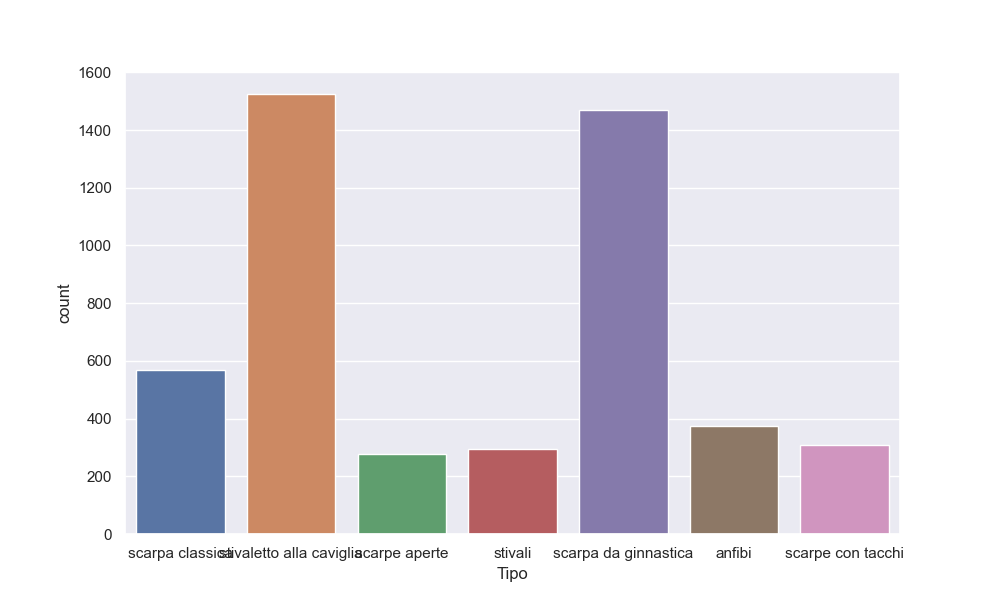
\includegraphics[scale=0.4]{countTipoShoes}
                    \end{center}
                    Per quanto riguarda gli attributi  \emph{Antiscivolo} e \emph{Impermeabile} sono stati imputati
                    logicamente sfruttando rispettivamente le colonne \emph{Insole} e \emph{Material}.
                    In breve, i valori di tali campi sono stati tradotti in italiano e, come per \emph{itemize}, i valori con significato simile sono stati
                    accorpati.
                    Inoltre, visto che alcuni righe contenevano un elenco di valori, sono state semplificate sostituendo l'elenco con il suo primo valore.
                    L'imputazione logica è stata effettuata sfruttando un dizionario python, per ulteriori dettagli si rimanda allo script
                    \href{https://github.com/frankzamma/NC22_WeatherStyle_classe03/blob/b8a2eb2de4f72fd37752e2c480e764e8797826f8/CreazioneDatasets/dataset_shoes/creazione_dataset_shoes.py}{creazione_dataset_shoes.py} sulla \href{https://github.com/frankzamma/NC22_WeatherStyle_classe03}{repository GitHub}
                    L'attributo \emph{stagione} è stato imputato utilizzando la colonna \emph{Tipo} costruita in precedenza: è stato costruito un dizionario
                    che per ogni tipo restituisce un insieme di stagioni possibili, tra queste ne viene scelta una casualmente.
                    L'attributo colore, siccome non poteva essere imputato in nessun modo e visto che non dipende in alcun modo dagli altri attributi
                    è stato imputato in maniera casuale scegliendo un valore tra i tre che abbiamo considerato: \emph{chiaro}, \emph{scuro} e \emph{colorato}.
                    \item Feature Scaling:\\
                    Non sono presenti dati numerici, di conseguenza, non è stato necessario applicare il feature scaling.
                    \item Feature Selection:
                    Le feature selezionate sono quelle citate precedentemente (\emph{Tipo}, \emph{Antiscivolo}, \emph{Impermeabile},\emph{Colore}, \emph{Stagione}), tutte le altre caratteristiche sono state rimosse.
                    \footnote{Nello script, la rimozione degli attributi che non vengono considerati o utilizzati per imputarne altri viene fatta all'inizio, per poter effettuare una rimozione dei valori e nulli e duplicati più efficiente}
                    \item Data Balacing\\
                    Il dataset presentava poche osservazioni relative a due tipologie di scarpe (\emph{Anfibi} e \emph{Stivali}), per questo motivo, è stato bilanciato aggiungendo dei dati generati per quei tipi tramite Google Sheet.
                \end{itemize}
                \subsection{Dataset meteo}
                Nella fase di data understanding, è stato illustrato che sono stati raccolti 14 diversi dataset con dati meteo per diverse città.
                Per poterli utilizzare, è stato necessario effettuare alcune operazioni su di essi:\\
                \begin{itemize}
                    \item Data Cleaning:\\
                    In questa fase, è stato necessario andare a ripulire la colonna \emph{WeatherCode} per 2 motivi:
                        \begin{enumerate}
                            \item i valori della colonna sono dei numeri ma in realtà tale colonna dovrebbe essere un variabile categorica
                            \item le condizioni meteo considerate sono troppe e alcune simili tra loro.
                        \end{enumerate}
                    Dunque, i valori di tale colonna sono stati sostituiti con dei nomi di condizioni meteo in italiano (Eg.
                    \emph{Soleggiato}) e i valori simili sono stati successivamente accorpati.
                    \item Feature Scaling:\\
                    Nel dataset sono presenti due colonne con valori numerici, cioè
                    \emph{Minimum Apparent Temperature} e \emph{Maximum Apparent Temperature},
                    ma sono già espressi nella stessa scala e dunque non si ritiene necessario effettuare una normalizzazione.
                    \item Feature Selection:\\
                    Le feature già presenti sono già molto buone, tuttavia è possibile fare dei miglioramenti
                    Le caratteristiche {Minimum Apparent Temperature} e \emph{Maximum Apparent Temperature}
                    possono essere sostituite da una singola colonna in cui si va ad inserire le medie tra i due valori.
                    Inoltre, la colonna \emph{Time} così com'è risulta essere poco utile, tuttavia è possibile utilizzarla per
                    creare una nuova colonna che contenga la stagione (Eg \emph{Autunno}, \emph{Agosto},\ldots).
                    \item Data Balacing:\\
                    Non è stato necessario effettuare un bilanciamento del dataset.
                \end{itemize}

                \subsection{La fusione dei dataset}
                Qui si parla di come è stata calcolata la variabile dipendente, facendo riferimento alla sezione dedicata
                alla formulazione del problema per il GA in particolare alla fitness

            \newpage
            \section{Modelling}
            Qui parliamo della tecnica di machine learning utilizzata, ovvero la regressione e dell'algoritmo utilizzato
                \subsection{La regressione}
                La regressione è un task di apprendimento supervisionato in cui l'obiettivo è quello di predire il valore
                di una variabile numerica (variabile dipendente) tramite l'utilizzo di un training set. La regressione
                porta alla costruzione di un modello, cioè di uno strumento che fa uso di un algoritmo di apprendimento
                (regressore) per predire i nuovi elementi sulla base del training set. Il regressore è una funzione matematica
                che descrive i dati e si effettua la distinzione tra regressione singola e multipla a seconda che ci sia
                rispettivamente una o più variabili indipendenti che aiutino nella predizione. Nel nostro caso, si parla di
                regressione multipla, in quanto ci sono più feature che contribuiscono nell'assegnazione di un punteggio ad
                un capo d'abbigliamento.
                \subsection{L'albero di regressione}
                Un \textbf{albero di regressione} segue sostanzialmente la logica di un albero decisionale con la principale
                differenza che anziché predire il valore di una variabile categorica, si occupa di predire il valore di
                una variabile numerica, apprendendo semplici regole inferite dai dati di training.
                \par \noindent L'algoritmo di addestramento mira quindi a creare un albero i cui nodi rappresentano un sottoinsieme
                di caratteristiche del problema e i cui archi rappresentano delle decisioni.
                \par \noindent Una volta ottenuto il modello sarà molto semplice comprendere il motivo di una predizione
                seguendo la path relativa agli input forniti.\\
                \par \noindent Nella sua istanza generale, che si tratti di un albero di decisione o di regressione, i
                passi dell'algoritmo saranno i seguenti:
                \begin{enumerate}
                    \item Posizionare la miglior caratteristica del training set come radice dell'albero.
                    \item Dividere il training set in sotto-insiemi. Ogni sotto-insieme dovrebbe essere composto di valori
                    simili per una certa caratteristica.
                    \item Ripetere gli step 1. e 2. fin quando non viene raggiunto un nodo foglia in ogni sotto-albero.
                \end{enumerate}
                \medskip
                \par \noindent Come ben sappiamo per poter piazzare la miglior caratteristica come radice dell'albero e/o
                di un sotto-albero, in modo che riesca a dividere bene le istanze del dataset, nei problemi di classificazione
                viene utilizzato l'\textbf{Information Gain}, mentre nei problemi di regressione abbiamo bisogno di un'indice
                diverso, dunque fa il suo ingresso l'\textbf{errore quadratico medio (MSE)}\footnote{come vedremo nelle
                successive sezioni, questo dipende fortemente da aspetti implementativi, talvolta si sceglie di utilizzare
                la \textbf{varianza} poiché quest'ultima permette di costruire un albero di regressione andando ad utilizzare
                variabili indipendenti che siano di natura numerica o nominale, nell'ultimo caso si vanno ad associare dei
                pesi ad ogni variabile rispetto alle frequenze degli attributi \cite{8}.}
                \[
                    MSE = \frac{1}{n}\sum_{i=1}^{n}(y_i - \overline{y_i})^2
                \]
                \\
                \par \noindent Supponiamo di avere un dataset come il seguente e di voler costruire un albero di regressione
                che preveda al meglio la Y data la X:
                \begin{center}
                    \begin{tabular}{| l | c |}      %barra tra una linea ed un altra
                        \hline                      %linee orizzontali
                        X & Y\\                     %le \\ indicano il termine riga
                        \hline
                        1 & 1\\
                        \hline
                        2 & 1.2\\
                        \hline
                        3 & 1.4\\
                        \hline
                        4 & 1.1\\
                        \hline
                        5 & 1\\
                        \hline
                        6 & 5.5\\
                        \hline
                    \end{tabular}
                \end{center}

                \newpage
                \par \noindent I passaggi che farà l'algoritmo saranno i seguenti:
                \begin{itemize}
                    \item \textbf{Primo passaggio:} ordina i dati nella colonna X (in questo caso sono già ordinati).
                    Prende la media delle prime due righe della colonna X, ovvero $(1+2)/3 = 1.5$, quindi divide il dataset
                    in due parti, la \textit{parte A} con $X < 1.5$ e la \textit{parte B} con $X \geq 1.5$.
                    \\Adesso farà la media di tutti i valori presenti in ambedue le parti e questi valori
                    definiranno l'output per l'albero di regressione in quel punto. Quindi calcola l'\textbf{MSE}
                    utilizzando i valori previsti $\overline{y_i}$ e i valori originali $y_i$, utilizzando le istanze
                    delle due parti.
                    \item \textbf{Secondo passaggio:} ripete il passaggio precedente con le successive righe della colonna
                    X, ovvero con i corrispettivi valori 2 e 3, 3 e 4, \ldots, fino all'$n-1$esimo numero, calcolandosi
                    l'MSE.
                    \item \textbf{Terzo passaggio:} una volta fatti i doverosi calcoli, l'algoritmo deciderà il punto in cui
                    dividere il dataset, ossia i valori che hanno permesso di ottenere un valore più basso in termini di MSE, questo decreterà
                    il punto di \textbf{radice}, dopodiché opererà allo stesso in maniera ricorsiva sui nodi figli, sino a raggiungere
                    una \textbf{foglia}\footnote{il numero minimo di istanze che compongono una foglia devono essere decisi durante
                    l'implementazione.}.
                \end{itemize}
                \medskip
                \begin{center}
                    \hspace*{5em}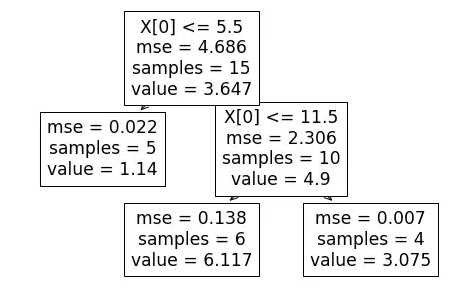
\includegraphics[scale=0.7]{albero}
                    \par \noindet Albero di regressione, immagine indicativa, non associata al dataset esposto.
                \end{center}
                \bigskip \bigskip
                \par \noindent \textbf{Cosa succede quando ci sono più variabili indipendenti?} In questo caso l'algoritmo
                procede allo stesso modo di come è stato descritto sopra con la differenza che i calcoli verrebbero fatti
                per ogni variabile indipendente. I punti che minimizzano l'MSE verrebbero calcolati per ogni variabile
                indipendente e verrebbero quindi scelti quelli meno intrinsechi all'errore.
                \\
                \par \noindent \textbf{Un grosso difetto...} gli alberi di decisione soffrono molto di \textbf{overfitting},
                ovvero tendono a fare un ragionamento eccessivamente complesso sui dati a disposizione, senza comprenderne
                l'essenza e la struttura. Questo rende gli alberi di decisone difficili da addestrare, nel caso dell'albero
                di regressione questo andrebbe avanti ricorsivamente nel tentativo di ridurre l'MSE, arrivando anche ad
                avere foglie con una sola istanza dove l'errore quadratico medio è nullo. Dunque è sempre consigliato
                specificare il numero minimo di istanze che deve avere un nodo foglia.

                \newpage
                \subsection{Ten-folds cross validation}
                Per addestrare e validare un modello di machine learning, si divide il dataset in due insiemi: training
                set (istanze che l'algoritmo utilizzerà per l'addestramento) e il test set (istanze per cui l'algoritmo
                addestrato dovrà predire il valore). Esistono diversi modi di dividere training e test set, tra cui
                considerare il 67\% del dataset come training set e il 33\% come test set. Nel caso di WeatherStyle,
                invece, è stata usata la \textit{convalida incrociata (o k-fold cross validation)}, con k=10.
                \\ \noindent La convalida incrociata è un metodo statistico che consiste nella ripetuta partizione e
                valutazione dell'insieme dei dati di partenza. Si basa sui seguenti step:
                \begin{itemize}
                    \item Si mischiano in maniera casuale i dati di partenza.
                    \item Si dividono i dati in dieci gruppi.
                    \item Per ogni gruppo, lo si considera come test set e si considerano gli altri nove come training set;
                    in questo modo, si addestra il modello con i dati del training set, si valutano le prestazioni del modello
                    e lo si elimina. Banalmente, nel nostro caso, il processo viene iterato dieci volte.
                \end{itemize}
                \par \noindent Da sottolineare che i processi di normalizzazione come feature selection e data balancing
                vengono effettuati ad ogni addestramento.
                \subsection{Valutazione delle metriche}
                Qui è possibile parlare delle metriche a cui ci siamo affidati, dei risultati ottenuti per ogni modello
                e inserire i grafici che mostrano la stima dell'errore rispetto alle predizioni fatte

            \section{Evaluation}
            Qui parliamo della sperimentazione empirica e dei risultati ottenuti
            Il risultato ottenuto non è da sottovalutare sicuramente per la non disponibilità dei dati.
            In particolare valutiamo

            \section{Deployment}
            Qui si parla leggermente dell'implementazione e delle scelte ingegneristiche per rendere il modello usabile
            quindi eventuali classi interfacce, ecc\ldots


    \part{Conclusioni e osservazioni}
        \chapter{Cosa scegliamo?}
            \section{Un confronto tra GA e ML}
                Quando conviene uno e quando conviene l'altro
            \section{Possiamo fare di meglio}
                Dopo aver quindi discusso dei pregi e dei difetti delle due tecniche di risoluzione da noi provate siamo
                venuti al capo e abbiamo pensato che si potesse ancora fare di meglio, in particolare nelle due prossime
                sotto-sezioni illustriamo ciò che potrebbe essere eventualmente fatto in futuro.
                \subsection{Usare il ML per il calcolo della funzione di fitness}
                Spiegare cosa si può fare
                \subsection{Usare un GA per costruire l'albero di regressione}
                Avendo provato due tecniche di risoluzione completamente diverse, abbiamo pensato alla possibilità di
                accorpare le due filosofie, in particolare potrebbe essere eliminata del tutto la fase di addestramento
                del modello di machine learning, sostituendo quindi la costruzione dell'albero di regressione mediante un
                algoritmo genetico.
                \par \noindent L'idea sarebbe quella di evolvere un \textbf{insieme di regole}, inizialmente
                generate in maniera pseudo-casuale per poi arrivare ad un punto sub-ottimale in cui avremo delle regole
                ben definite che descriveranno tutti i possibili percorsi dell'albero di regressione.


    % sezione dedicata ai riferimenti bibliografici
    \begin{thebibliography}{9} % meno di 10, 99 meno di 100 e così via...
        \bibitem{1}
        Jenetics, Java Genetic Alghorithm Library,
        \url{https://jenetics.io/}.

        \bibitem{2}
        Weka, Waikato Environment for Knowledge Analysis,
        \url{https://www.cs.waikato.ac.nz/ml/weka/}.

        \bibitem{3}
        Kaggle,
        \url{https://www.kaggle.com}

        \bibitem{4}
        pandas,
        \url{https://pandas.pydata.org/docs/}

        \bibitem{5}
        seaborn,
        \url{https://seaborn.pydata.org/}

        \bibitem{6}
        dataset maglie e pantaloni,
        \url{https://github.com/justjess678/clothes-scraper.git}

        \bibitem{7}
        dataset scarpe
        \url{https://www.kaggle.com/datasets/ramu237/shoes-dataset}

        \bibitem{8}
        Analisi della varianza,
        \url{https://it.wikipedia.org/wiki/Analisi_della_varianza}

        \bibitem{9}
        Open-meteo
        \url{https://open-meteo.com/}
    \end{thebibliography}

\end{document}